
\chapter{Results and Future Work}

\section{Experimental results}

For the evaluation of the proposed method, we conducted experiments using the \textit{SummitXL} of \textit{Robotnik} equipped with notably a laser scanne and IMU sensors.
The test environment was a room with a size of approximately $ 7 \times 6 $ meters.
We moved slowly the robot to minimize the noise in the data collected by the IMU.


\begin{figure}[H]
    \centering
    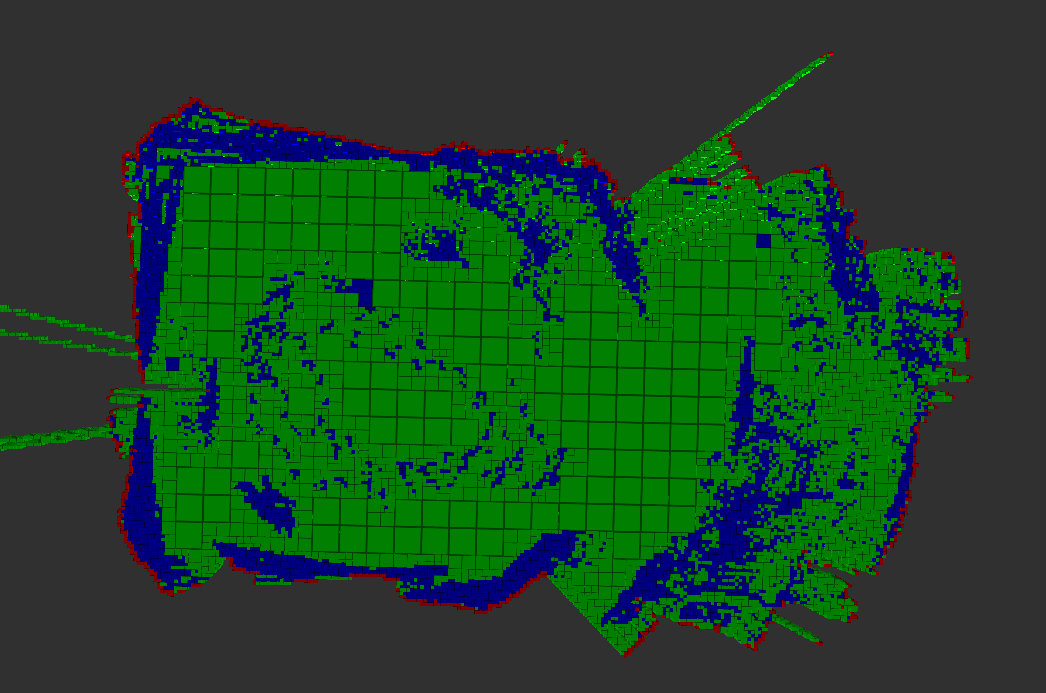
\includegraphics[width=\textwidth]{images/top_screenshot.png}
    \caption{Top view of the octomap generated by our program in the P.E.R.M.I.S. environment. The gray area represents the unknown space, the green area represents the free space, and the red area represents the occupied space. Only the major probability values are shown.}
\end{figure}

In the P.E.R.M.I.S. environment, with the \textit{SummitXL} robot, we obtained the following results:

\begin{itemize}
    \item We see a coherent representation of the environment in the octomap, the boundaries of the room are defined.
    \item The moving objects are detected, in the figure the circle made of blue points represents a person moving around.
    \item Near the boundaries of the room, the program detects a lot of conflicts, this can be explained by the fact that the robot is moving and the IMU is not perfect.
    \item The attenuation could be useful to detect the moving objects, indeed, when occupied cells are surrounded by conflicts cells, it's often a fixed object but when the conflict disappears, it's often a moving object.
    \item The program is able to run in real-time, around 15 Hz and can be significantly improved by reducing the resolution.
\end{itemize}

